\section{圏と公理}\label{chap-2-category-and-axiom}
	\begin{define}\label{def-category}
    ある圏$\cat{C}$は以下で定義される対象集合$\obj{C}$と、任意の二対象$A,B$に対するそれぞれの射集合$\arset{C}{A}{B}$、合成の演算$\circ$によって定義する。また圏は以下に示す公理を満たさなければならない。
		\begin{quote}
			\begin{mydescription}
			\item[対象] 圏はある集合$\obj{C}$を持つ必要がある。\\
			この集合を\textbf{対象集合}と呼ぶことにし、対象集合の要素を\textbf{対象}と呼ぶことにする。
			\item[射] 任意の対象$A,B$に対してある集合$\arset{C}{A}{B}$を持つ必要がある。
      またこのような集合を\textbf{射集合}と呼ぶことにし、射集合の要素を\textbf{射}と呼ぶことにする。\\
			このような射集合は任意の二対象$A,B$に対して存在することに注意してほしい。二対象$A,B$の間に射が存在しない場合の射集合は空集合となる。
			\\また$f\in\arset{C}{A}{B}$である時$\mor{f}{A}{B}$と書く。このとき$f$に対する$A$を\textbf{始域}、$B$を\textbf{終域}と呼び、射から対象への二つの演算$\dom,\cod$を用い$\dom(f)=A$、$\cod(f)=B$と表す。\\

			ある対象$A,B,C$、ある射$\mor{f}{A}{B}$、$\mor{g}{A}{C}$、$\mor{h}{C}{B}$について考えるとき、以下のような図式を用いて説明を行う。
			\begin{center}
				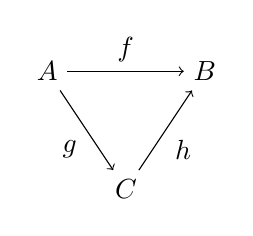
\begin{tikzpicture}[auto]
					\node (a) at (0, 0) {$A$};
					\node (b) at (2, 0) {$B$};
					\node (c) at (1, -1.5) {$C$};
					\draw[->] (a) to node {$f$}(b);
					\draw[->] (a) to node[swap] {$g$}(c);
					\draw[->] (c) to node[swap] {$h$}(b);
				\end{tikzpicture}
			\end{center}
			\item[射の合成]~\\ ある射$f,g$が$\cod(f)=\dom(g)$を満たす、つまり$\mor{f}{X}{A}$、$\mor{g}{A}{Y}$であるようなとき、ある射$\mor{g\circ f}{X}{Y}$が存在し、このような射を\textbf{合成射}と呼ぶ。
			射をつなげる、という直感に反して合成射の射の順序が射の向きと逆であることに注意してほしい。

			射$h,g$の合成$h\circ g$は次のように表せる。
			また対象$A$と対象$B$の間の射は一つとは限らないので、必ずしも$h\circ g=f$が成り立つわけではない。
			\begin{center}
				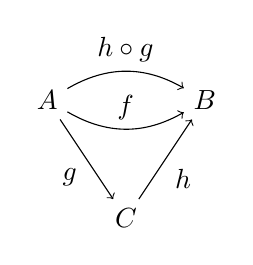
\begin{tikzpicture}[auto]
					\node (a) at (0, 0) {$A$};
					\node (b) at (2, 0) {$B$};
					\node (c) at (1, -1.5) {$C$};
					\draw[->] (a) to[bend right=30] node {$f$}(b);
					\draw[->] (a) to[bend right=-30] node {$h\circ g$}(b);
					\draw[->] (a) to node[swap] {$g$}(c);
					\draw[->] (c) to node[swap] {$h$}(b);
				\end{tikzpicture}
			\end{center}
			このような操作は任意の対象$A,B,C$における二変数の写像\[\mor{\circ}{\arset{\cat{C}}{B}{C}\times\arset{\cat{C}}{A}{B}}{\arset{\cat{C}}{A}{C}}\]
			で表せる。また厳密には写像$\circ$は任意の対象$A,B,C$の組み合わせごとに個別に存在する。
			\item[恒等射の存在] \textbf{恒等射}と呼ばれる特別な射$\mor{id_A}{A}{A}$が任意の対象に存在する。
			\begin{center}
				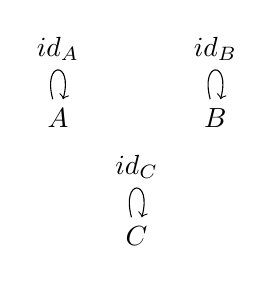
\begin{tikzpicture}[auto]
					\node (a) at (0, 0) {$A$};
					\node (b) at (2, 0) {$B$};
					\node (c) at (1, -1.5) {$C$};
					\draw[->,loop above ,looseness=10] (a) to node{$id_A$}(a);
					\draw[->,loop above ,looseness=10] (b) to node{$id_B$}(b);
					\draw[->,loop above ,looseness=10] (c) to node{$id_C$}(c);
				\end{tikzpicture}
			\end{center}
			\item[結合律] 結合則$h\circ (g\circ f)=(h\circ g)\circ f$が合成可能な任意の射$f,g,h$で成り立つ。
				\begin{center}
				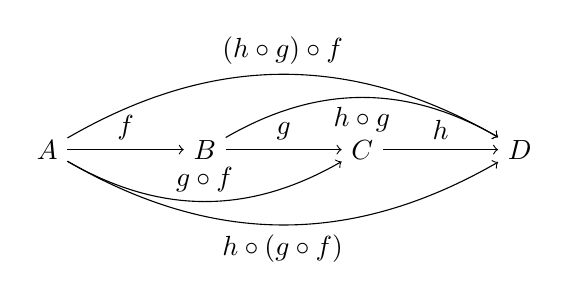
\begin{tikzpicture}[auto]
					\node (a) at (0, 0) {$A$};
					\node (b) at (2, 0) {$B$};
					\node (c) at (4, 0) {$C$};
					\node (d) at (6, 0) {$D$};
					\draw[->] (a) to node {$f$}(b);
					\draw[->] (b) to node {$g$}(c);
					\draw[->] (c) to node {$h$}(d);
					\draw[->] (a) to[bend right=30] node {$g\circ f$}(c);
					\draw[->] (a) to[bend right=30] node[swap] {$h\circ(g\circ f)$}(d);
					\draw[->] (b) to[bend left=30] node[swap] {$h\circ g$}(d);
					\draw[->] (a) to[bend left=30] node {$(h\circ g)\circ f$}(d);
				\end{tikzpicture}
			\end{center}
			\item[単位元律]~\\ 任意の対象$A$と対応する恒等射$\mor{id_A}{A}{A}$、任意の射$\mor{f}{X}{A}$、$\mor{g}{A}{Y}$において\[id_A\circ f=f,\ g\circ id_A=g\]が成り立つ。

			恒等射をある射に合成しても、合成する前の射と等しくなることから、直感的に恒等射は何も行わない射のように考えられる。

			\begin{center}
				\begin{tikzpicture}[auto]
					\node (x) at (0, 0) {$X$};
					\node (a) at (2, 0) {$A$};
					\node (y) at (4, 0) {$Y$};
					\draw[->] (x) to node {$f$}(a);
					\draw[->,loop above, looseness=20] (a) to node {$id_A$}(a);
					\draw[->] (a) to node {$g$}(y);
				\end{tikzpicture}
				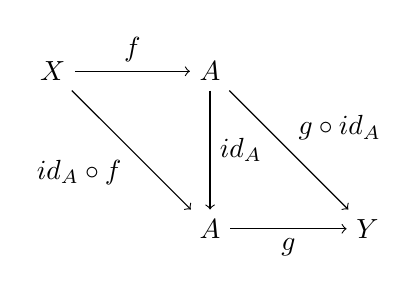
\begin{tikzpicture}[auto]
					\node (a) at (0, 0) {$X$};
					\node (b) at (2, 0) {$A$};
					\node (b') at (2, -2) {$A$};
					\node (c) at (4, -2) {$Y$};
					\draw[->] (a) to node {$f$}(b);
					\draw[->] (b) to node {$id_A$}(b');
					\draw[->] (b') to node[swap]  {$g$}(c);
					\draw[->] (a) to node[swap]  {$id_A\circ f$}(b');
					\draw[->] (b) to node {$g\circ id_A$}(c);
				\end{tikzpicture}
			\end{center}
		\end{mydescription}
			\end{quote}
	\end{define}
	\begin{define}[圏の同一性]\label{def-equation-of-categories}
		圏$\cat{A,B}$が\textbf{同一}、$\cat{A}=\cat{B}$であるとは、対象の集合、射の集合、合成の演算が集合、写像として等しいということである。
	\end{define}
	次に圏の例として集合の圏を挙げる。
	\begin{define}[集合の圏]\label{def-category-of-sets}
		圏$\cat{Set}$を以下の要素から構成する。
		\begin{quote}
			\begin{mydescription}
				\item[対象] $\obj{Set}$を小さな集合の集合とする。

				「小さい」は自己言及を避けるための条件であり、実際に$\obj{Set}$は大きい集合となるため$\obj{Set}$には含まれない。
				\item[射] 二対象$A,B$に対する射集合$\arset{Set}{A}{B}$を小さな集合$A$から小さな集合$B$への写像の集合とする。

				また紛らわしい場合を除いて小さい集合を集合と呼ぶことにする。

				集合の圏では一般的な圏とは違い、対象を集合として元をとることができる。
				そして同対象間に射が二つあったとき、二つの写像が等しいかどうかを元の対応関係で確かめることができる。
				つまり、二つの写像$\mor{f,g}{A}{B}$と集合$A$の任意の元$a$に対して、\[f(a)=g(a)\]ならば$f=g$が成り立つ、ということである。以降は元の対応関係を用いて集合の圏の射である写像を定義していく。

				\item[射の合成]  二つの写像$\mor{f}{A}{B}$、$\mor{g}{B}{C}$の\textbf{合成写像}$\mor{g\circ f}{A}{C}$を$A$の任意の元$a$に対して\[(g\circ f)(a)=g(f(a))\]となるように定義する。

				集合の圏は一般的な圏とは違い、元の対応関係を調べるだけで射が等しくなることを示せる。
				\item[恒等射の存在] 任意の集合$A$に対する恒等射$id_A$を$A$の任意の元$a$に対して\[id_A(a)=a\]となるように定義する。
				\item[結合律] 任意の写像$\mor{f}{A}{B}$、$\mor{g}{B}{C}$、$\mor{h}{C}{D}$に対して$h\circ(g\circ f)=(h\circ g)\circ f$が成り立つことを示せばよい。
				それぞれ合成写像の定義を用いて
				\begin{align*}
					((h\circ g)\circ f)(a)&=(h\circ g)(f(a))\\
					&=h(g(f(a)))\\
					&=h((g\circ f)(a))\\
					&=(h\circ(g\circ f))(a)
				\end{align*}
				となり、写像の合成では結合律が成り立つ。
				\item[単位元律] 任意の集合$A$と対応する恒等写像$id_A$、任意の写像$\mor{f}{X}{A}$、$\mor{g}{A}{Y}$において\[(id_A\circ f)(x)=f(x),\ (g\circ id_A)(a)=g(a)\]が成り立つことを示せばよい。
				\begin{align*}
					(id_A\circ f)(x)&=id_A(f(x))&\text{(写像の合成の定義)}\\
					&=f(x)&\text{{(恒等写像の定義)}}\\
					(g\circ id_A)(a)&=g(id_A(a))&\text{(写像の合成の定義)}\\
					&=g(a)&\text{{(恒等写像の定義)}}
				\end{align*}
				よって単位元律が成り立つ。
			\end{mydescription}
		\end{quote}
	\end{define}
	
	集合の圏の射である写像は、任意の元が同じ元に対応することによって射が等しいことを示せたが、一般の圏ではそうは限らない。そもそも対象の元を取ることができるとは限らないし、元の対応関係が一致していても同じ射であるとも限らない。

	集合の圏を集合によって定義したが以降で使用する集合としての性質は、元の対応関係により射が等しいことを示せること以外はほとんど使用しない。仮に使用したとしても、直ちに圏論的な定義に置き換える。